\chapter{Model}
\label{sec:privacy_metrics}
In this chapter we introduce our model and the privacy metrics used in order to quantify the privacy provisions of an adblocker.

\section{Request graph}
\label{sec:graph_definition}
We model the tracking profile of a user $U$ through third parties as an undirected graph $G=(E,V)$, where $E$ are edges, and $V$ vertices. A vertex $V_S$ represents a domain and is connected to another vertex $V_T$ through an edge $E$, if and only if at least one request has been sent from $V_S$ to $V_T$. In that case, $V_S$ is the \textit{source} of the request and $V_T$ the \textit{target} of the request.

In the following, we use the term \textit{third-party request} (TPR) to denote the requests that are sent to a target domain $T$ that differs from the source domain $S$ and corresponds to a graph edge $E$ between the nodes $V_S$ and $V_T$. On the contrary, the requests whose source and target coincide are designated as \textit{first-party requests} (FPR) and are not taken into consideration for the construction of $G$, since no information leaks to third parties and hence they do not bring about further risks for user's privacy. The source and the target domain are referred to as \textit{first-party domain} (FPD) and \textit{third-party domain} (TPD) and correspond to FPD and TPD graph nodes, $V_S$ and $V_T$, respectively.

We augment \emph{G} by incorporating the legal relationship between third party domains. Two TPD, belong to the same legal entity if they belong to the same incorporation (e.g., Google Inc.) and are thus combined into one vertex, resulting in a hierarchical graph (cf. Figure~\ref{fig:graph}). Finally we attribute each legal entity to a geographical location (effectively capturing which countries capture how many third party domains). Given \emph{G}, we evaluate the respective privacy provisions based on the following metrics.

\begin{figure}[tb!]
  \centering 
  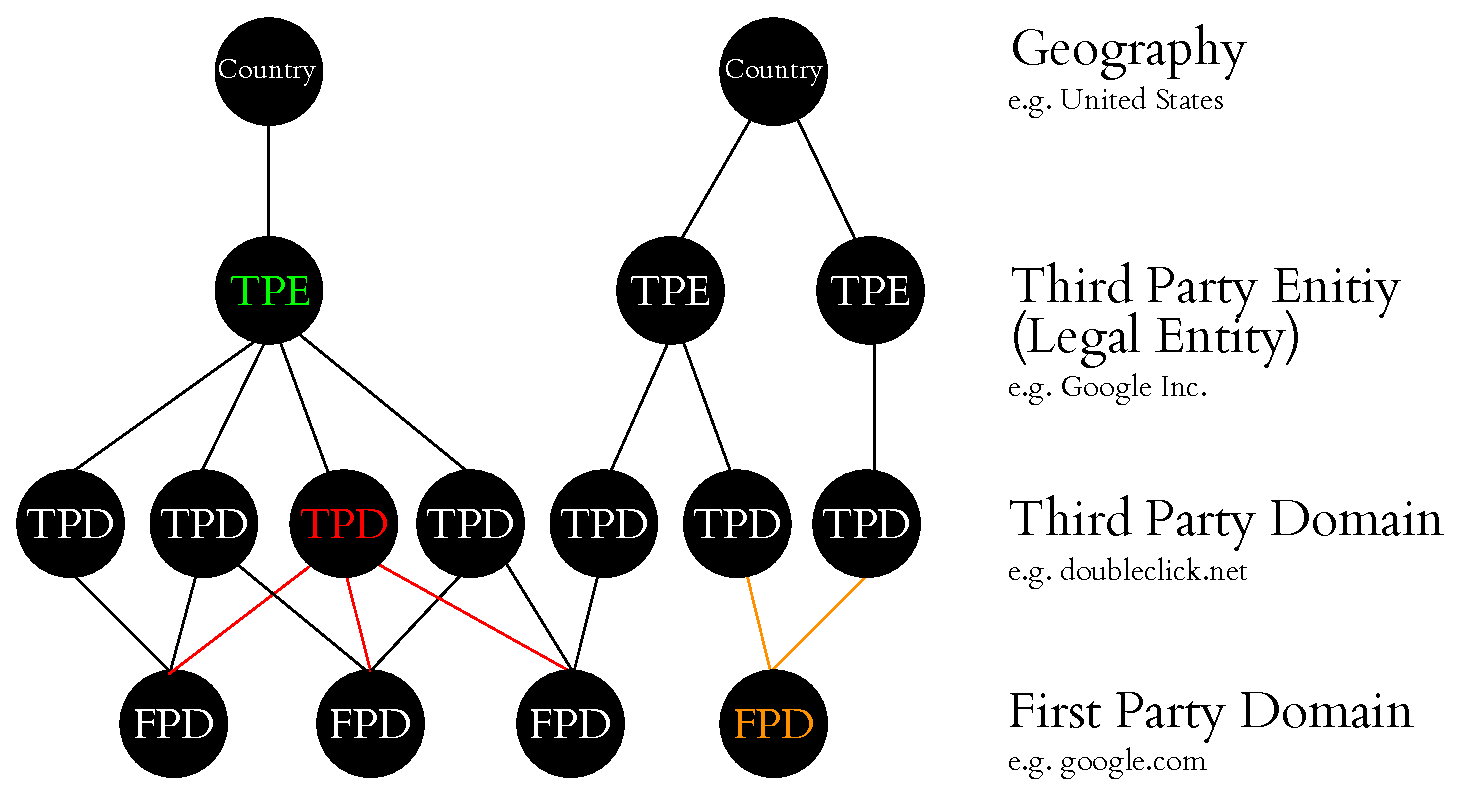
\includegraphics[width=\textwidth]{figures/graph.eps}
  \caption{Components of our model. The colored TPD has a node degree of~3, the colored FPD has a node degree of~2. The colored TPE spans all its child TPD nodes and hence has a degree of~3.}
  \label{fig:graph}
\end{figure}

\section{Privacy Metrics}
In the following section we elaborate our privacy metrics to quantify the privacy provisions of a web adblocker. We categorize the privacy metrics in \emph{(i)} first order relationships, \emph{(ii)} graph metrics and \emph{(iii)} the temporal change.

\subsection{First Order Relationships}
We outline in the following two primary privacy metrics that are captured via the first order relationship between FPDs and TPDs.

\paragraph{Degree of First Party Domain}
The degree of a FPD node of graph $G$ refers to the number of TPDs that it has sent at least one third-party request to. That is, the more edges a FPD node has --- or, equivalently, the more third parties loaded by a first-party --- the more third parties are able to track the web-browsing history of a user. The comparison of the FPD-node degrees therefore provides a metric to directly evaluate the adblocker's impact on privacy~\cite{ruffel2015}.

\paragraph{Degree of Third Party Domain}
The degree of a TPD node can be directly translated into the number of first-party websites that a particular third party exchanges information with and potentially tracks. Clearly, the more often a third party is accessed over the user's series of websites $S_U$, the less privacy the user experiences from this particular third party~\cite{englehardt}. To exemplify this statement, let's assume that a third party is requested by only one of the first-party websites $S_U$ visited by $U$. This third party will in this case learn that the user has accessed the respective first party, but has a limited view of their browsing behavior. If the third party, however, is requested by over 80\% of the user's visited websites, $S_U$, the third party will likely be able to recover 80\% of the web behavior of $U$.

We capture this privacy notion by assessing the degree of the TPD nodes in the graph $G$ so as to evaluate the improvement that the ad-blocking software can achieve.

\subsection{Graph metric}
In addition to the outlined privacy metrics, we consider the graph density of $G$. Since an edge on the graph $G$ represents a partial tracking relationship between a third and a first party, we expect that the denser the graph $G$, the more information can be retrieved by third parties -- or equivalently, can leak to third parties -- with respect to the browsing behavior of the user. We observe that the denser $G$ is, the more third parties are likely able to track the user $U$. The graph density therefore allows to reason about the possible privacy improvements by the respective ad-blocking software. For undirected graphs, the graph density is commonly defined as:
\begin{equation}
\label{eq:density}
D = \frac{2 |E|}{|V|(|V|-1)}
\end{equation}

Note that we cannot achieve the maximum density of 1, because the first parties in $G$ are not directly connected (cf. definition in Section~\ref{sec:graph_definition}).

\subsection{Temporal change}
The formerly presented metrics only allow us to reason about the privacy provisions of the advertisement blocking software at a given time $t$. The advertisement industry, however, operates dynamically by using e.g., new advertisement techniques and new third party URLs. Within our model we therefore capture the temporal change of the first order relationships (degree of third and first party respectively) and the graph density metric. We do so by evaluating the respective metrics over a time-span and are thus able to judge about the temporal stability of the proposed metrics.

\paragraph{Blacklist changes}
In addition to the temporal changes of our metrics, we as well capture when an adblocker updates its blacklist --- we thus observe the update behaviour of the respective adblocker instances, an indicator of how fast the adblocker adapts to the changing advertisement environment.

\section{Beyond Domains}
The described metrics only capture domain based knowledge --- domain knowledge however does not provide any information about the underlying legal entity (i.e., operating company) or the geographical location of the domain (i.e., its country). Since the URL information, however, does not encapsulate many aspects of the respective web infrastructure and resulting privacy risks, we augment the graph $G$, by incorporating, legal entities, their respective geographical location, the influence of \emph{do not track} (DNT) headers and the difference between mobile and desktop clients.

\subsection{Legal entity}
\label{sec:legal_entity}
Instead of focusing on the URL of a third party, we link the third parties based on their respective owner information. Third parties such as \url{doubleclick.net} and \url{google.com} for example are both owned by the same entity Google Inc. Their collusion therefore seems more likely, and affects the privacy of a web user $U$ more significantly, than if both were belonging to two different legal entities. By incorporating the legal relation among third party domains, we therefore capture a more realistic privacy leakage through user web surf activity.

\subsection{Geographical location}
After having mapped the TPD's to legal entities, we further assign a geographical location to the TPD. This allows our model to capture the geographical distribution of the TPDs and thus infer which geographical countries have for instance the greatest TPD.

\subsection{DNT influence}
Modern web browsers allow its user to set the \emph{do not track} HTTP header option, to express their personal preference regarding tracking to each server they request content from, thereby allowing recipients of that preference to adjust tracking behavior, accordingly~\cite{dnt}. It remains the sole responsibility of the web server to respect the request of its clients. Almost 10\% of the Firefox users have enabled this option on their desktop browsers in 2014~\cite{dnt_state_firefox}. In order to evaluate to which extent the DNT header has an influence on our proposed metrics we as well include the DNT option in our model.

\subsection{User agent}
The usage of mobile devices for web browsing has recently witnessed a steady growth~\cite{mobile_usage}. As a consequence, an ever increasing number of websites has been adapting to the demands of the mobile user agents. Because of the dimensions and the reduced-bandwidth requirements of the mobile devices, the structure and content of the web pages has to be adjusted accordingly and the advertising content could not remain unaffected by these limitations.

To investigate the effects of user agents from a privacy-related perspective, we consider this parameter in the design of the experimental evaluation and simulate several mobile-device instances by setting the HTTP header \textit{User-Agent} accordingly.